\chapter{Inflationary Cosmology}
\label{chap:cos}

\section{Introduction}
\label{sec:cos:intro}

\section{Conventions}
\label{sec:cos:conventions}


\begin{enumerate}
  \item I work using a metric with a positive signature $(+,-,-,-)$.
  \item Fourier transforms are written with an overloaded notation, and defined so that Fourier synthesis carries the factors of $2\pi$:
    \begin{equation}
      f(\vk) = \int_{-\infty}^{\infty} d^3\vx\: e^{-i \vk\cdot\vx} f(\vx) \qquad f(\vx) = \int_{-\infty}^{\infty} \frac{d^3\vk}{(2\pi)^3}\: e^{i \vx\cdot\vk} f(\vk).
      \label{eqn:cos:fourier_transform}
    \end{equation}
  \item I work in natural units so that 
    \begin{equation}
      c = \hbar = G = k_B = 1,
      \label{eqn:cos:natural_units}
    \end{equation}
    but retain the reduced Planck mass for clarity:
    \begin{equation}
      \m = \frac{1}{8\pi G}.
      \label{eqn:cos:reduced_planck_mass}
    \end{equation}
    
\end{enumerate}


\section{Differential geometry}
\label{sec:cos:differential_geometry}

The application and understanding of Einstein's theory of general relativity requires an understanding of curved spacetime.

\begin{figure}
  \centerline{%
    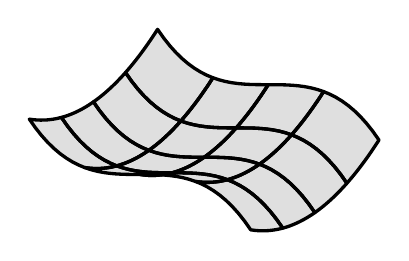
\begin{tikzpicture}[
    x=(215:2em/sqrt 2), y=(0:2em), z=(90:2em),
    declare function={f(\x,\y)=((\x-3)^2+(-\y+3)^3)/8+3;}, 
  very thick, line join=round]
%  \draw [-stealth, black!75] (0,0,0) -- (5,0,0) node [below left] {$x$};
%  \draw [-stealth, black!75] (0,0,0) -- (0,5,0) node [below right] {$y$};
%  \draw [-stealth, black!75] (0,0,0) -- (0,0,5) node [right] {$z$};

  \foreach \x in {1,...,4}
  \foreach \y in {1,...,4}{
    \draw [black, fill=black, fill opacity=0.125, 
    domain=0:1, samples=10, variable=\t] 
    plot (\x+\t, \y, {f(\x+\t,\y)}) -- 
    plot (\x+1, \y+\t, {f(\x+1,\y+\t)}) -- 
    plot (\x+1-\t, \y+1, {f(\x+1-\t,\y+1)}) --
    plot (\x, \y+1-\t, {f(\x,\y+1-\t)}) -- cycle;
  }
\end{tikzpicture}

  }
  \caption{\label{fig:cos:differenial_geometry}}
\end{figure}

\subsection{Coordinates}
Curved spacetime is a collection of events (or points) $p$ in a manifold $\mathcal{M}$. Semi-global patches of it may have their events labelled with coordinates $x^\mu = x^\mu(p)$, which are always ``upstairs'' indexed. Since we are in $1+3$ spacetime, typically, $\mu=0$ will denote a time-like coordinate, and $\mu=1,2,3$ space-like coordinates.

\subsection{Vectors}
This coordinate system defines a {\em contravariant\/} set of basis vectors at each point $\ve_\mu = \ve_\mu(p)$. Here the basis vector $\ve_\mu(p)$ is tangent to the coordinate curve:
\begin{equation}
  \gamma^\mu = \{x^\nu=\mathrm{const} : \mu\ne\nu\},
  \label{eqn:cos:coordinate_curve}
\end{equation}
at the point $p$.\footnote{Experienced readers will know that this notion is normally regarded as far from trivial.}
  Vectors at {\em at a given point\/} $p$ form a vector space which may be summed and scaled. Thus, a general vector $\vv$ may be written as a linear combination of basis vectors $\vv = v^\mu \ve_\mu$, where we use Einstein's summation convention that repeated upstairs and downstairs indices should be summed over. In addition, these vectors are equipped with a dot-product $\vv\cdot\vw$ which encapsulates the geometry of the vectors; namely spacetime angles and magnitudes. If a coordinate system is chosen, then:
\begin{equation}
  \vv\cdot\vw = (v^\mu\ve_\mu)\cdot(w^\nu\ve_\nu) = v^\mu (\ve_\mu\cdot\ve_\nu)w^\nu =  v^\mu g_{\mu\nu} w^\nu
  \label{eqn:cos:dot_product}
\end{equation}
where 
\begin{equation}
  g_{\mu\nu} = \ve_\mu\cdot\ve_\nu
  \label{eqn:cos:metric_def}
\end{equation}
is the {\em metric}, and is simply the dot product at a given point, expressed in a specific coordinate system.

Once a dot product is defined, it is convenient to define a set of {\em covariant\/} basis vectors $\{\ve^\mu\}$ via:
\begin{equation}
  \ve^\mu \cdot \ve_\nu = \delta^\mu_\nu 
  \qquad\Leftrightarrow\qquad
  \ve^\mu = g^{\mu\nu} \ve_\nu,
  \label{eqn:cos:covariant_basis}
\end{equation}
where $g^{\mu\nu}$ is the upstairs version of \eqref{eqn:cos:metric_def}, and by simple linear algebra is the matrix inverse of $g_{\mu\nu}$. Now that a dot product is defined, the covariant basis vector $\ve^\mu$ can be thought of as orthogonal to the coordinate surface $x^\mu=\mathrm{const}$. Materials scientists should recognise the covariant basis as simply the reciprocal basis. 

We can choose to write vectors in either the covariant or contravariant basis:
\begin{equation}
  \vv=v^\nu \ve_\nu = v_\mu \ve^\mu 
  \qquad\Rightarrow\qquad
  v_\mu = g_{\mu\nu} v^\nu.
  \label{eqn:cos:covariant_vector}
\end{equation}
The metric can therefore be used to ``raise'' or ``lower'' indices of vectors. The fact that the metric performs this operation should be intuitively obvious, since raised or lowered indexed vectors correspond to placing the vector in the covariant or contravariant coordinate system, whose definition \eqref{eqn:cos:covariant_basis} is defined via the dot-product.

\subsection{Tensors}
A Tensor $T$ is a multi-linear mapping of vectors onto a scalar at a given point:
\begin{align}
  T 
  &= 
  T(\va,\:\vb,\ldots,\:\vz)
  &
  \nonumber
  \\
  &= 
  T(a^\alpha\ve_\alpha,\:b^\beta\ve_\beta,\ldots,z^\zeta\ve_\zeta)  
  &\text{vectors in coordinate basis}
  \nonumber
  \\
  &= 
  a^\alpha b^\beta \ldots z^\zeta \: 
  T(\ve_\alpha,\:\ve_\beta,\:\ldots,\:\ve_\zeta)  
  &\text{apply multi-linearity}
  \nonumber
  \\
  T_{\alpha,\beta,\ldots,\zeta} 
  &=  
  T(\ve_\alpha,\:\ve_\beta,\:\ldots,\:\ve_\zeta)
  &\text{define a new set of numbers}
  \nonumber
  \\
  \Rightarrow\qquad
  T
  &= 
  a^\alpha b^\beta \ldots z^\zeta \: 
  T_{\alpha,\beta,\ldots,\zeta}
  &
  \nonumber
\end{align}
Upstairs components of a vector are defined similarly. It is interesting (although not surprising) that the metric is also a tensor, albeit a very special one which defines the geometry. The mapping is coordinate independent, but components are produced when a specific coordinate basis is chosen for each ``slot'' (each of which may be covariant or contravariant).

A mapping of a rank $m$ tensor onto a rank $n$ tensor may be produced from a rank $m+n$ tensor by simply leaving $n$ of the slots blank. In this sense, a vector can be considered as a rank $1$ tensor, its linear action defined by the dot product.

\subsection{Calculus}




\section{Einstein's gravity}
\label{sec:cos:einsteins_gravity}

Einstein's gravity can be effectively summarised using the Einstein-Hilbert action formalism. An action $S$ is written as a general relativistic integral over a Lagrangian density $\mathcal{L}$:\footnote{This should not be confused with a likelihood, also denoted with $\lik$.}
\begin{equation}
  S = \int d^4 x \sqrt{|g|} R
  \label{eqn:cos:action}
\end{equation}
where $g=\det(g_{\mu\nu})$ is the determinant of the metric, and $R$ is the Ricci scalar, defined by
\begin{align}
  R &= R^\mu_\mu \label{eqn:cos:ricci_scalar_def} \\
  R_{\mu\nu} &= R^\rho_{\mu\rho\nu} \label{eqn:cos:ricci_tensor_def} \\
  R_{\mu\nu} &= R^\rho_{\mu\rho\nu} \label{eqn:cos:riemann_tensor_def} \\
  R^\rho_{\sigma\mu\nu} &= \partial_\mu\Gamma^\rho{}_{\nu\sigma}
    - \partial_\nu\Gamma^\rho{}_{\mu\sigma}
    + \Gamma^\rho{}_{\mu\lambda}\Gamma^\lambda{}_{\nu\sigma}
    - \Gamma^\rho{}_{\nu\lambda}\Gamma^\lambda{}_{\mu\sigma}
\end{align}

We define the action:
\begin{equation}
  S = S_G + S_m
  \label{eqn:cos:action}
\end{equation}
where
\begin{equation}
  S_G = \int \frac{1}{2}
  \label{<++>}
\end{equation}<++>

\section{Background}
\label{sec:background}

\clearpage{}

We denote a general action via
\begin{equation}
  S_I = \int d^4x\sqrt{|g|}\mathcal{L}_I,
  \label{eqn:general_action}
\end{equation}
where $\mathcal{L}_I$ is the {\em Lagrangian density}. We work in natural units $\hbar=c=1$ and set the reduced Planck mass $m_\mathrm{p} = {(8\pi G)}^{-1/2} = 1$. Dots denote differentiation with respect to cosmic time $\dot{f}\equiv \frac{d}{dt}f$, and primes denote differentiation with respect to conformal time $\prm{f}\equiv\frac{d}{d\eta}f$.

We begin by briefly summarising the classical theory of cosmological perturbations for a general scalar field, before discussing the quantisation of such a theory


\subsection{The classical action}
\label{sec:inflation}
Consider~\cite{Baumann+2009} a canonical scalar field $\phi$ minimally coupled to gravity $S= S_G + S_\phi$ with:
\begin{equation}
  \mathcal{L}_G = \frac{1}{2}R, 
  \qquad
  \mathcal{L}_\phi = \frac{1}{2}g^{\mu\nu}\nabla_\mu\phi\nabla_\nu\phi - V(\phi),
  \label{eqn:action}
\end{equation}
Extremising this action with respect to the fields $\phi$ and $g_{\mu\nu}$ recovers the Klein-Gordan and Einstein equations respectively:
\begin{align}
  \left( g^{\mu\nu}\nabla_\mu\nabla_\nu + \frac{dV}{d\phi} \right) \phi &= 0,
  \label{eqn:klein_gordon}\\
  G_{\mu\nu}\equiv R_{\mu\nu}-\frac{1}{2}g_{\mu\nu}R&= T_{\mu\nu},
  \label{eqn:einstein}
\end{align}
where the stress-energy tensor is:
\begin{equation}
  T_{\mu\nu} = \nabla_\mu\phi \nabla_\nu\phi - \frac{1}{2}g_{\mu\nu} \nabla_\alpha\phi \nabla^\alpha\phi +g_{\mu\nu} V(\phi).
  \label{eqn:SET}
\end{equation}

In cosmology, we assume that at zeroth order both the metric $g_{\mu\nu}$ and scalar field $\phi$ are homogeneous and isotropic. Applying these assumptions to equations~(\ref{eqn:klein_gordon})~\&~(\ref{eqn:einstein}), we find:
\begin{align}
  \dot{H}+H^2 &= -\frac{1}{3}\left( \dot{\phi}^2 - V(\phi) \right),
  \label{eqn:Raychaudhuri}\\
  0&=\ddot{\phi} + 3H\dot{\phi} + \frac{dV}{d\phi},
\end{align}
where the Hubble parameter $H = \dot{a}/a$.
